\documentclass[12pt]{article}
\usepackage[dot, autosize, outputdir="dotgraphs/"]{dot2texi}
\usepackage{tikz}
\usetikzlibrary{shapes}
\usepackage[utf8]{inputenc}
\usepackage{amsmath}
\usepackage{mathtools}
\usepackage{amsfonts}
\usepackage{lastpage}
\usepackage{pdfpages}
\usepackage{gauss}
\usepackage{fancyvrb}
\usepackage{fancyhdr}
\usepackage{graphicx}
\pagestyle{fancy}
\fancyfoot[C]{\footnotesize Page \thepage\ of 5}
\DeclareGraphicsExtensions{.pdf,.png,.jpg}
\title{Oversætter}
\author{Nikolaj Dybdahl Rathcke}
\chead{Nikolaj Dybdahl Rathcke (rfq695)}

\begin{document}
\section*{Oversætter - Week 3}

\subsection*{1 - Parameter-Passing Conventions}
We have the following program
\begin{verbatim}
void main() {                  int f(int a, int b, int c) {
  int x = 5;  int y = 2;         a = b + c;
  int r = f(x, y, x);            b = c - b;
  print(r);                      c = c + a;
  print(x); print(y);            return (a + b + c);
}                              }
\end{verbatim}

\subsubsection*{1a}
What is printed if call-by-value is used? Explain briefly why.\\
\\
It prints $r=22$, since this is the return value with the formal parameters.\\
It prints $x=5$ since the argument in $f$ do not match those in $main$.\\
It prints $y=2$ for the same reason as above.

\subsubsection*{1b}
What is printed if call-by-reference is used? Explain briefly why.\\
\\
It prints $r=33$ since the values $a$ and $c$ are the same, so when $a$ is changed, so is $c$.\\
It prints $x=14$ for the same reason as stated above.\\
It prints $y=5$ for the same reason.

\subsubsection*{1c}
What is printed if call-by-value-result is used? Explain briefly why.\\
\\
It prints $r=22$ since it is the same result as in (1a).\\
It prints $x=12$ or $x=7$ depending on the update order, since $x$ is updated to either $a$ or $c$ just before the callee returns.\\
It prints $y=3$ for the same reason as above.

\newpage

\subsection*{2 - Dynamic and Static Scoping}
We have the following program
\begin{verbatim}
int x = 5; // global x

void g()      { print(x);                    }
void h(int y) { int x = y + 2; g();          }
void f(int x) { if (x == 4) g(); else h(x);  }
\end{verbatim}

\subsubsection*{2a}
With static  scoping, what would $f(4)$ and $f(7)$ print, respectively? Explain briefly why.\\
\\
$f(4)$ and $f(7)$ will both print $x=5$ because $g$ will both refer to the global variable $x$.

\subsubsection*{2b}
With dynamic scoping, what would `f(4)' and `f(7)' print, respectively? Explain briefly why.\\
\\
$f(4)$ will print $x=4$ because $x$ is set when the function is called with the argument $x$ and then tested as a boolean. Then $g$ will refer to the $x$ from the function call.\\
$f(7)$ will print $x=9$ since $x$ is set in $h$ which is more recent.

\subsubsection*{2c}
Explain briefly how one can implement dynamic scoping in Paladim's interpreter.\\
\\
Everytime a variable is declared or changed, it will be pushed onto a stack and will then look through the stack in a top-down manner. If the variable exists, it 'overwrites' it by popping the value when returning to the callee. Thus, it always has the most recent value for each variable.

\subsection*{3 - Type Inference}

\subsubsection*{3a}
Explain the main steps by which Paladim's type checking infers the type of each subexpression of:
\begin{verbatim}
        chr( read() ) = read()
\end{verbatim}
Also state the types of the two (calls to) read.\\
\\
Since the chr function is int $\rightarrow$ char, this means that the first read must be of type int and the second read must be of type char.

\subsubsection*{3b}
Show how to apply the unification algorithm discussed in class to unify the types below and say who alpha, beta and the unified type are after unification:
\begin{verbatim}
list(int) * list(alpha)     and      alpha * beta
\end{verbatim}
$ $\\
We use the unification algorithm and get\\
\begin{center}
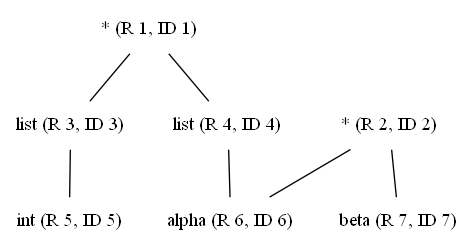
\includegraphics[scale=0.6]{graph1}
\end{center}
\newpage
Applying rule 4
\begin{center}
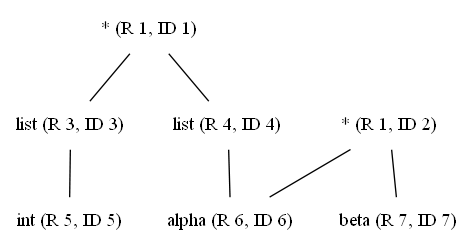
\includegraphics[scale=0.6]{graph2}
\end{center}
Applying rule 3
\begin{center}
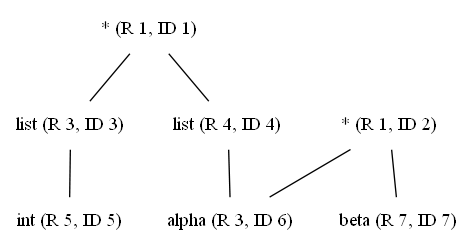
\includegraphics[scale=0.6]{graph3}
\end{center}
Applying rule 3
\begin{center}
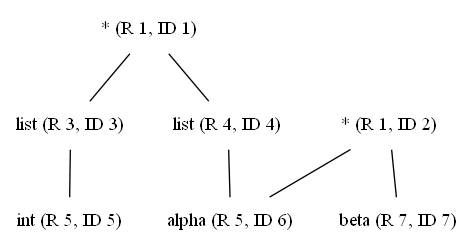
\includegraphics[scale=0.6]{graph4}
\end{center}
Applying rule 3
\begin{center}
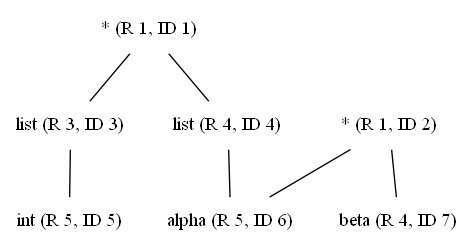
\includegraphics[scale=0.6]{graph5}
\end{center}
Applying rule 3
\begin{center}
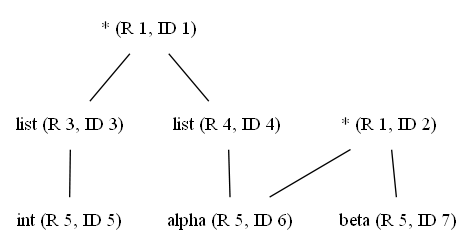
\includegraphics[scale=0.6]{graph6}
\end{center}
And the type is then: list(int) * list(int)
\end{document}
